\subsection{Módulo genérico de las señales ferroviarias}
	\label{sec:ACG_sig}
	
	El módulo \textit{Signals} (ver Figura \ref{fig:GeneralSystem}) es el encargado de implementar el funcionamiento de las señales ferroviarias. El ACG determina cuantos caminos posibles existen utilizando como punto de partida la señal ferroviaria a implementar. Cada uno de los caminos posibles influirá en el comportamiento de la señal ferroviaria. Para determinar cual es el único camino posible, el ACG implementa los puertos y conexiones a cada uno de los elementos ferroviarios involucrados con esa señal y hasta dos señales futuras, para todos sus caminos. En base a los estados reportados por estos elementos ferroviarios, el módulo \textit{Signals} determinará cuál es el camino activo y su señal ferroviaria quedará definida totalmente. El diagrama de bloques de la máquina de estados finitos con camino de datos diseñado para lograr este objetivo se muestra en la Figura \ref{fig:SIG_module}.
	
	\begin{figure}[H]
		\centering
		\includegraphics[width=1\textwidth]{Figuras/SIG_module}
		\centering\caption{FSMD del módulo genérico de \textit{Signals}.}
		\label{fig:SIG_module}
	\end{figure}
	
	Como fue explicado en la Sección \ref{sec:signals}, el aspecto de una señal ferroviaria será rojo si el conjunto de \textit{netElements} al que habilita circular la formación ferroviaria se encuentra ocupado. Si se encontrasen desocupados, su aspecto dependerá del aspecto de la señal siguiente. Cuál es la señal siguiente dependerá del estado actual de toda la infraestructura entre la señal analizada y dos señales consecutivas. El comportamiento del aspecto de una señal ferroviaria se define en la red de Petri de la Figura \ref{fig:SIG_Petri}.
	
	\begin{figure}[H]
		\centering
		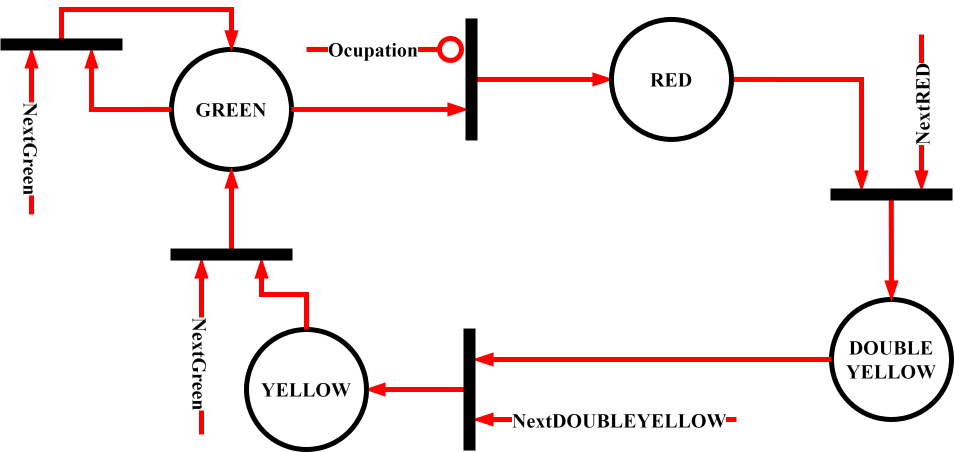
\includegraphics[width=1\textwidth]{Figuras/SIG_petri}
		\centering\caption{Red de Petri del modelo dinámico de \textit{Signals}.}
		\label{fig:SIG_Petri}
	\end{figure}
	
	La red de Petri ilustrada en la Figura \ref{fig:SIG_Petri} es una simplificación de la implementación real, en la que solamente se ilustra un único cambio de estado entre un aspecto y otro. De haber ilustrado todas las transiciones entre, por ejemplo, el aspecto rojo y amarillo, el aspecto rojo y verde, o el aspecto rojo consigo mismo, entonces la cantidad de transiciones sería tres veces mayor.
	
	Teniendo en cuenta el modelo simplificado, una señal ferroviaria depende de sí misma solo si la sección a la que protege se encuentra ocupada, en cuyo caso su aspecto será rojo. En caso contrario, si la sección se encuentra libre, dependerá del aspecto de la señal siguiente: si la señal siguiente es roja, el aspecto de la señal analizada será doble amarillo; si la señal siguiente es doble amarilla, el aspecto de la señal analizada será amarillo; si la señal siguiente es amarilla, el aspecto de la señal analizada será verde y, finalmente, si la señal siguiente es verde, el aspecto de la señal analizada también lo será.
	
	Las señales ferroviarias no pueden cambiar su aspecto una vez que se encuentran enclavadas, salvo para adoptar un aspecto mas restrictivo, para garantizar un mayor nivel de seguridad.